\documentclass[aspectratio=169, 10pt]{beamer}

% ---------- Tema y colores ----------
\usetheme{default}
\usecolortheme{default}
\setbeamertemplate{navigation symbols}{}
\setbeamertemplate{footline}[frame number]
\setbeamertemplate{frametitle continuation}{}

\definecolor{StanfordRed}{RGB}{140,21,21}
\definecolor{LightGray}{RGB}{240,240,240}
\definecolor{AccentGreen}{RGB}{0,130,100}
\definecolor{UCMBlue}{RGB}{4, 171, 226}
\definecolor{UCMNavy}{RGB}{20, 65, 134}

\definecolor{mitblue}{RGB}{20, 65, 134}
\definecolor{mitgray}{RGB}{169, 169, 169}

\setbeamercolor{frametitle}{fg=white, bg=UCMBlue}
\setbeamercolor{title}{fg=white}
\setbeamercolor{author}{fg=white}
\setbeamercolor{institute}{fg=white!80}
\setbeamercolor{structure}{fg=UCMBlue}
\setbeamercolor{block title}{bg=UCMBlue!15!white, fg=UCMBlue}
\setbeamercolor{block body}{bg=LightGray}
\setbeamercolor{block title alerted}{bg=StanfordRed!15!white, fg=StanfordRed}
\setbeamercolor{block body alerted}{bg=LightGray}
\setbeamercolor{alerted text}{fg=UCMBlue}

\setbeamerfont{frametitle}{series=\bfseries, size=\large}
\setbeamerfont{title}{series=\bfseries, size=\LARGE}
\setbeamerfont{block title}{series=\bfseries}

% ---------- Paquetes ----------
\usepackage[utf8]{inputenc}
\usepackage[T1]{fontenc}
\usepackage[provide=*,spanish]{babel}
\usepackage{amsmath, amssymb}
\usepackage{graphicx}
\usepackage{tikz}
\usepackage{pgfplots}
\pgfplotsset{compat=1.18}
\usetikzlibrary{arrows, arrows.meta, shapes, shapes.geometric, positioning,
	fit, calc, matrix, chains, decorations.pathreplacing,
	backgrounds, shadows}
\usepackage{booktabs}
\usepackage{array}
\usepackage{xcolor}
\usepackage{multicol}
\usepackage{tcolorbox}
\tcbuselibrary{skins, breakable}
\usepackage{fontawesome5}

% ---------- Comandos \'utiles ----------
\providecommand{\R}{\mathbb{R}}
\newcommand{\V}{\mathcal{V}}
\newcommand{\tok}[1]{\texttt{#1}}
\newcommand{\W}[1]{\mathbf{W}_{\textrm{#1}}}
\newcommand{\bvec}[1]{\mathbf{b}_{\textrm{#1}}}
\newcommand{\good}{{\color{AccentGreen}\faCheck}}
\newcommand{\bad}{{\color{StanfordRed}\faTimes}}

\newcommand{\formula}[1]{%
	\begin{tcolorbox}[colback=UCMBlue!8, colframe=UCMBlue, arc=4pt,
		boxsep=2pt, left=6pt, right=6pt, top=3pt, bottom=3pt]
		#1
	\end{tcolorbox}
}

\tcbset{codebox/.style={colback=LightGray, colframe=UCMNavy, arc=3pt, boxsep=1pt, left=4pt, right=4pt, top=2pt, bottom=2pt}}

% ---------- Portada ----------
\title{\textbf{Embeddings Vectoriales y Redes Neuronales Recurrentes}}
\subtitle{De vectores de palabras a modelos de secuencias}
\author{Sergio Hern\'andez, PhD\\ shernandez@ucm.cl}
\institute{
	\begin{tikzpicture}[scale=0.42, every node/.style={transform shape}]
		\foreach \i/\y in {1/0,2/1,3/2}{\node[circle,draw=white,fill=white!20,minimum size=4mm] (i\i) at (0,\y){};}
		\foreach \i/\y in {1/-0.5,2/0.5,3/1.5,4/2.5}{\node[circle,draw=white,fill=white!35,minimum size=4mm] (h\i) at (2,\y){};}
		\foreach \i/\y in {1/0.5,2/1.5}{\node[circle,draw=white,fill=white!50,minimum size=4mm] (o\i) at (4,\y){};}
		\foreach \a in {1,2,3}\foreach \b in {1,2,3,4}{\draw[white,opacity=0.5] (i\a)--(h\b);}
		\foreach \a in {1,2,3,4}\foreach \b in {1,2}{\draw[white,opacity=0.5] (h\a)--(o\b);}
	\end{tikzpicture}
	\\ \textbf{Mag\'ister en Data Science --- Universidad Cat\'olica del Maule}}
\date{}

\begin{document}
% --- T\'itulo ---
{
	\setbeamertemplate{background}{
		\begin{tikzpicture}[remember picture, overlay]
			\fill[UCMBlue] (current page.south west) rectangle (current page.north east);
			\fill[UCMBlue!70!black, opacity=0.5]
			(current page.south west) -- ++(0,3) -- ++(18,0) -- cycle;
			\foreach \i in {1,...,40}{
				\fill[white, opacity=0.04]
				({random()*17}, {random()*10}) circle ({random()*0.3});
			}
		\end{tikzpicture}
	}
	\begin{frame}[plain]
		\vspace{1.2cm}
		\titlepage
		\begin{tikzpicture}[remember picture, overlay]
			\node[white, opacity=0.15, font=\fontsize{80}{80}\selectfont]
			at (current page.east) [xshift=-2.4cm] {$\mathbf{h}_t$};
		\end{tikzpicture}
	\end{frame}
}

% =================================================================
\section{Introducci\'on}

\begin{frame}{¿D\'onde Estamos?}

	\begin{columns}[T]
		\begin{column}{0.5\textwidth}
			\begin{block}{Clase 3.1}
				\small
				\begin{itemize}
					\item Texto $\to$ tokens $\to$ \'indices.
					\item Representaciones por conteo: BoW, $n$-gramas, TF-IDF.
					\item Embeddings preentrenados: word2vec, GloVe, BERT.
				\end{itemize}
			\end{block}

			\begin{alertblock}{Lo que falta}
				\small
				Todas esas representaciones de \emph{documento} \textbf{agregan} palabras (suma, promedio) y \textbf{pierden el orden}:
				\begin{itemize}
					\item ``el perro mordi\'o al hombre'' $=$ ``el hombre mordi\'o al perro''.
					\item ``no es bueno, es excelente'' vs.\ ``es bueno, no es excelente''.
				\end{itemize}
			\end{alertblock}
		\end{column}

		\begin{column}{0.47\textwidth}
			\begin{block}{Esta clase}
				\small
				\begin{enumerate}
					\item \textbf{Embeddings vectoriales} como capa de una red: \texttt{nn.Embedding}, \texttt{EmbeddingBag}, vectores preentrenados.
					\item \textbf{Modelos de secuencias}: autorregresivos, Markov, modelos de lenguaje, perplejidad.
					\item \textbf{Redes recurrentes} (RNN): estado oculto, entrenamiento con BPTT, gradientes que se desvanecen o explotan.
					\item \textbf{LSTM, GRU}, RNN bidireccionales y multicapa.
					\item Clasificaci\'on de AG\_NEWS con RNN y LSTM (Lab 3.2).
				\end{enumerate}
			\end{block}
		\end{column}
	\end{columns}

\end{frame}

% =================================================================
\section{Embeddings Vectoriales}

\begin{frame}{La Capa de Embedding}

	\begin{columns}[c]
		\begin{column}{0.5\textwidth}
			\small
			Multiplicar un vector one-hot $\mathbf{e}_i \in \{0,1\}^{|\V|}$ por una matriz $\mathbf{E} \in \R^{|\V|\times d}$ selecciona la fila $i$:
			\formula{\centering $\mathbf{e}_i^\top \mathbf{E} = \mathbf{E}[i,:] \in \R^{d}$}
			\begin{itemize}
				\item Una capa \texttt{Linear} sin sesgo sobre one-hot $\equiv$ \textbf{tabla de b\'usqueda}.
				\item \texttt{nn.Embedding(vocab\_size, d)} recibe \textbf{\'indices} enteros y devuelve filas: no materializa el one-hot.
				\item $\mathbf{E}$ se entrena por retropropagaci\'on como cualquier peso, o se inicializa con vectores preentrenados.
				\item $d \ll |\V|$: de 95\,810 dimensiones (BoW de AG\_NEWS) a 32--300.
			\end{itemize}
		\end{column}

		\begin{column}{0.47\textwidth}
			\centering
			\resizebox{\linewidth}{!}{%
	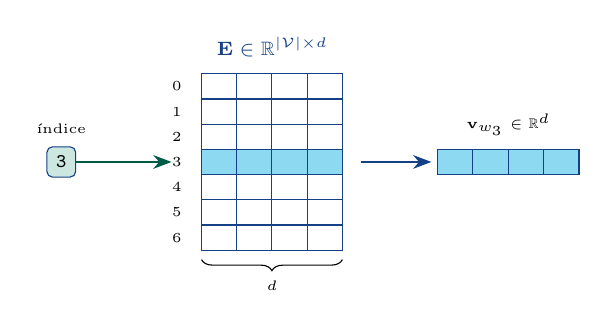
\begin{tikzpicture}[
					cell/.style={draw=UCMNavy, minimum width=0.45cm, minimum height=0.32cm, inner sep=0pt, font=\tiny},
					hl/.style={cell, fill=UCMBlue!45}
				]
				% matriz E
				\foreach \r in {0,...,6}{
					\foreach \c in {0,...,3}{
						\ifnum\r=3
							\node[hl] at (\c*0.45, -\r*0.32) {};
						\else
							\node[cell, fill=white] at (\c*0.45, -\r*0.32) {};
						\fi
					}
					\node[font=\tiny, anchor=east] at (-0.35, -\r*0.32) {\r};
				}
				\node[font=\scriptsize\bfseries, text=UCMNavy] at (0.68, 0.5) {$\mathbf{E}\in\R^{|\V|\times d}$};
				\draw[decorate, decoration={brace, amplitude=4pt, mirror}] (-0.22,-2.2) -- (1.57,-2.2) node[midway, below=4pt, font=\tiny] {$d$};
				% indice
				\node[draw=UCMNavy, fill=AccentGreen!20, font=\scriptsize\ttfamily, rounded corners=2pt] (idx) at (-2.0, -0.96) {3};
				\node[font=\tiny, above=1pt of idx] {\'indice};
				\draw[-{Stealth}, thick, AccentGreen!70!black] (idx.east) -- (-0.6, -0.96);
				% salida
				\foreach \c in {0,...,3}{\node[hl] at (3.0+\c*0.45, -0.96) {};}
				\draw[-{Stealth}, thick, UCMNavy] (1.8, -0.96) -- (2.7, -0.96);
				\node[font=\tiny, above] at (3.68, -0.75) {$\mathbf{v}_{w_3} \in \R^d$};
			\end{tikzpicture}}

			\vspace{0.3cm}

			{\small Una oraci\'on de $T$ tokens se convierte en una matriz $T \times d$: \textbf{una fila por posici\'on}, el orden se conserva.}
		\end{column}
	\end{columns}

\end{frame}

\begin{frame}[fragile,shrink]{Clasificador con Embeddings (Lab 3.4)}

	\begin{columns}[T]
		\begin{column}{0.53\textwidth}
			\begin{tcolorbox}[codebox]
\scriptsize
\begin{verbatim}
class EmbedClassifier(torch.nn.Module):
    def __init__(self, vocab_size, embed_dim,
                 num_class):
        super().__init__()
        self.embedding = torch.nn.Embedding(
                             vocab_size, embed_dim)
        self.fc = torch.nn.Linear(embed_dim,
                                  num_class)

    def forward(self, x):          # x: (B, T)
        x = self.embedding(x)      # (B, T, d)
        x = torch.mean(x, dim=1)   # (B, d)
        return self.fc(x)          # (B, 4)
\end{verbatim}
			\end{tcolorbox}

			\begin{tcolorbox}[codebox]
\scriptsize
\begin{verbatim}
def padify(b):   # rellena con 0 hasta el maximo
    v = [encode(x[1]) for x in b]
    l = max(map(len, v))
    return (torch.LongTensor([t[0]-1 for t in b]),
            torch.stack([F.pad(torch.tensor(t),
                (0, l-len(t)), value=0) for t in v]))
\end{verbatim}
			\end{tcolorbox}
		\end{column}

		\begin{column}{0.44\textwidth}
			\begin{block}{Arquitectura}
				\formula{\centering $\hat{\mathbf{y}} = \mathrm{softmax}\Big(\mathbf{W}\,\frac{1}{T}\sum_{t=1}^{T}\mathbf{v}_{w_t} + \mathbf{b}\Big)$}
				\small
				El promedio de embeddings es una ``BoW densa'': sigue \textbf{ignorando el orden}.
			\end{block}

			\begin{block}{Resultado (lab)}
				\small
				$d=32$, 25\,000 ejemplos: exactitud $\approx 76\%$ (frente a $\approx 86\%$ de BoW con 95\,810 entradas). Con m\'as \'epocas se acerca a $\sim$90\%.
			\end{block}

			\begin{alertblock}{Relleno}
				\small
				Los minilotes necesitan secuencias del mismo largo: se rellenan con el \'indice 0. Los ceros \emph{s\'i} entran al promedio.
			\end{alertblock}
		\end{column}
	\end{columns}

\end{frame}

\begin{frame}[fragile]{Secuencias de Largo Variable: \texttt{EmbeddingBag}}

	\begin{columns}[T]
		\begin{column}{0.5\textwidth}
			\small
			En lugar de rellenar, se concatenan todas las secuencias del lote en un \textbf{\'unico vector} y se guardan los \textbf{desplazamientos} (\emph{offsets}) donde empieza cada una.

			\vspace{0.2cm}
			\centering
			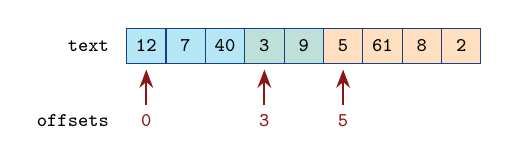
\begin{tikzpicture}[
					c/.style={draw=UCMNavy, minimum width=0.5cm, minimum height=0.45cm, font=\scriptsize\ttfamily, inner sep=0pt},
				]
				\foreach \v [count=\i from 0] in {12,7,40,3,9,5,61,8,2}{
					\pgfmathsetmacro{\col}{\i<3 ? "UCMBlue!30" : (\i<5 ? "AccentGreen!25" : "orange!25")}
					\node[c, fill=\col] at (\i*0.5, 0) {\v};
				}
				\node[font=\scriptsize, anchor=east] at (-0.35,0) {\texttt{text}};
				\foreach \o/\x in {0/0, 3/1.5, 5/2.5}{
					\draw[-{Stealth}, thick, StanfordRed] (\x, -0.75) -- (\x, -0.3);
					\node[font=\scriptsize\ttfamily, StanfordRed] at (\x, -0.95) {\o};
				}
				\node[font=\scriptsize, anchor=east] at (-0.35,-0.95) {\texttt{offsets}};
			\end{tikzpicture}

			\raggedright
			\begin{tcolorbox}[codebox]
\scriptsize
\begin{verbatim}
self.embedding = torch.nn.EmbeddingBag(
        vocab_size, embed_dim)   # mode='mean'
def forward(self, text, off):
    return self.fc(self.embedding(text, off))
\end{verbatim}
			\end{tcolorbox}
		\end{column}

		\begin{column}{0.47\textwidth}
			\begin{tcolorbox}[codebox]
\scriptsize
\begin{verbatim}
def offsetify(b):
    x = [torch.tensor(encode(t[1])) for t in b]
    o = [0] + [len(t) for t in x]
    o = torch.tensor(o[:-1]).cumsum(dim=0)
    return (torch.LongTensor(
                [t[0]-1 for t in b]),
            torch.cat(x),  # texto concatenado
            o)             # inicios
\end{verbatim}
			\end{tcolorbox}

			\begin{itemize}
				\small
				\item \texttt{EmbeddingBag} = b\'usqueda + agregaci\'on (\texttt{mean}, \texttt{sum}, \texttt{max}) en una sola operaci\'on.
				\item Sin relleno: no se desperdicia memoria ni c\'omputo, y el relleno no contamina el promedio.
				\item Exactitud similar ($\approx 75\%$ en 25\,000 ejemplos).
			\end{itemize}
		\end{column}
	\end{columns}

\end{frame}

\begin{frame}[fragile,shrink]{Embeddings Preentrenados}

	\begin{columns}[T]
		\begin{column}{0.5\textwidth}
			\small
			Los embeddings aprendidos s\'olo para clasificar no tienen por qu\'e reflejar \textbf{significado}. Se pueden importar vectores entrenados con word2vec o GloVe sobre corpus enormes (clase 3.1):

			\begin{tcolorbox}[codebox]
\scriptsize
\begin{verbatim}
import gensim.downloader as api
w2v = api.load('word2vec-google-news-300')
w2v.most_similar('neural')
# neuronal 0.78, neurons 0.73,
# neural_circuits 0.73, neuron 0.72, ...
\end{verbatim}
			\end{tcolorbox}

			\begin{tcolorbox}[codebox]
\scriptsize
\begin{verbatim}
E = torch.zeros(vocab_size, 300)
for i, w in enumerate(vocab.get_itos()):
    if w in w2v: E[i] = torch.tensor(w2v[w])
    else:        E[i] = torch.randn(300) * 0.1
net.embedding.weight.data = E
net.embedding.weight.requires_grad = False
\end{verbatim}
			\end{tcolorbox}
		\end{column}

		\begin{column}{0.47\textwidth}
			\begin{block}{Decisiones de dise\~no}
				\small
				\begin{itemize}
					\item \textbf{Congelar} $\mathbf{E}$: pocos datos etiquetados, se conserva la sem\'antica general.
					\item \textbf{Ajustar} $\mathbf{E}$: muchos datos, se adapta al dominio (riesgo de olvidar).
					\item Palabras fuera del vocabulario preentrenado: inicializaci\'on aleatoria o subpalabras (fastText).
					\item El tokenizador debe ser \textbf{compatible} con el del modelo preentrenado (min\'usculas, frases unidas por \texttt{\_}).
				\end{itemize}
			\end{block}

			\begin{alertblock}{L\'imite}
				\small
				Con embeddings est\'aticos y un promedio, la red sabe \emph{qu\'e} palabras hay pero no \emph{en qu\'e orden}. Necesitamos un modelo de \textbf{secuencias}.
			\end{alertblock}
		\end{column}
	\end{columns}

\end{frame}

% =================================================================
\section{Modelos de Secuencias}

\begin{frame}{Datos Secuenciales}

	\begin{columns}[T]
		\begin{column}{0.5\textwidth}
			\small
			Hasta ahora las entradas ten\'ian \textbf{largo fijo} (tablas, im\'agenes de $28\times28$). Texto, audio, video y series de tiempo son \textbf{secuencias} $\mathbf{x}_1, \ldots, \mathbf{x}_T$ de largo variable, con $\mathbf{x}_t \in \R^d$.

			\vspace{0.2cm}

			\begin{itemize}
				\item Las secuencias completas se suponen i.i.d.; los elementos \emph{dentro} de una secuencia son dependientes.
				\item La secuencia puede estar en la entrada, en la salida o en ambas.
			\end{itemize}
		\end{column}

		\begin{column}{0.47\textwidth}
			\begin{block}{Tipos de tareas}
				\scriptsize
				\renewcommand{\arraystretch}{1.15}
				\begin{tabular}{@{}>{\raggedright}p{2.2cm}>{\raggedright\arraybackslash}p{3.3cm}@{}}
					\toprule
					\textbf{Forma} & \textbf{Ejemplo} \\
					\midrule
					fijo $\to$ secuencia & descripci\'on de im\'agenes \\
					secuencia $\to$ fijo & sentimiento, t\'opico (AG\_NEWS) \\
					secuencia $\to$ secuencia alineada & etiquetado POS, NER \\
					secuencia $\to$ secuencia no alineada & traducci\'on, di\'alogo \\
					\bottomrule
				\end{tabular}
			\end{block}
		\end{column}
	\end{columns}

	\vspace{0.3cm}

	\centering
	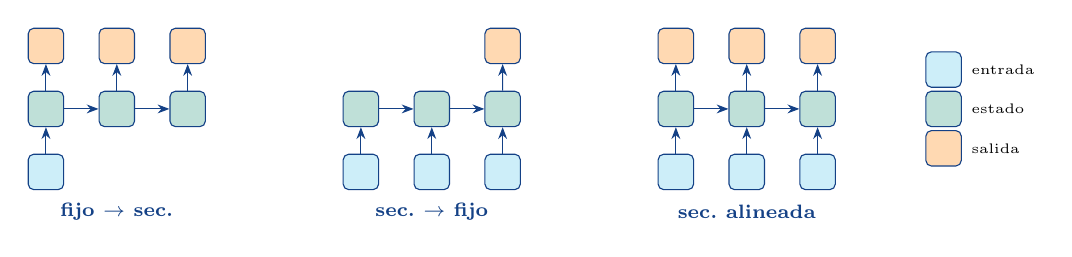
\begin{tikzpicture}[
			b/.style={draw=UCMNavy, fill=UCMBlue!20, rounded corners=2pt, minimum size=0.45cm},
			r/.style={draw=UCMNavy, fill=AccentGreen!25, rounded corners=2pt, minimum size=0.45cm},
			o/.style={draw=UCMNavy, fill=orange!30, rounded corners=2pt, minimum size=0.45cm},
			a/.style={-{Stealth[length=1.5mm]}, UCMNavy}
		]
		\foreach \g/\lab/\ins/\outs in {0/{fijo $\to$ sec.}/1/3, 4/{sec. $\to$ fijo}/3/1, 8/{sec. alineada}/3/3}{
			\foreach \i in {1,2,3}{
				\node[r] (h\g\i) at (\g+\i*0.9, 0) {};
				\ifnum\i>1 \pgfmathtruncatemacro{\j}{\i-1}\draw[a] (h\g\j) -- (h\g\i); \fi
			}
			\node[font=\scriptsize\bfseries, text=UCMNavy] at (\g+1.8, -1.3) {\lab};
		}
		% fijo -> sec
		\node[b] at (0.9,-0.8) {}; \draw[a] (0.9,-0.57) -- (h01);
		\foreach \i in {1,2,3}{\node[o] at (\i*0.9,0.8) {}; \draw[a] (h0\i) -- (\i*0.9,0.57);}
		% sec -> fijo
		\foreach \i in {1,2,3}{\node[b] at (4+\i*0.9,-0.8) {}; \draw[a] (4+\i*0.9,-0.57) -- (h4\i);}
		\node[o] at (6.7,0.8) {}; \draw[a] (h43) -- (6.7,0.57);
		% sec alineada
		\foreach \i in {1,2,3}{\node[b] at (8+\i*0.9,-0.8) {}; \draw[a] (8+\i*0.9,-0.57) -- (h8\i);
			\node[o] at (8+\i*0.9,0.8) {}; \draw[a] (h8\i) -- (8+\i*0.9,0.57);}
		\node[b, label={[font=\tiny]right:entrada}] at (12.3,0.5) {};
		\node[r, label={[font=\tiny]right:estado}] at (12.3,0) {};
		\node[o, label={[font=\tiny]right:salida}] at (12.3,-0.5) {};
	\end{tikzpicture}

\end{frame}

\begin{frame}{Modelos Autorregresivos}

	\begin{columns}[T]
		\begin{column}{0.52\textwidth}
			\small
			Por la regla de la cadena, cualquier distribuci\'on conjunta se factoriza como
			\formula{\centering $P(x_1,\ldots,x_T) = P(x_1)\displaystyle\prod_{t=2}^{T} P(x_t \mid x_{t-1},\ldots,x_1)$}
			Problema: el n\'umero de entradas del condicional \textbf{crece con $t$}. Dos soluciones:

			\begin{block}{1. Ventana fija (Markov de orden $\tau$)}
				\small
				Condicionar s\'olo en $x_{t-1},\ldots,x_{t-\tau}$. Con $\tau = 1$:
				\[
					P(x_1,\ldots,x_T) = P(x_1)\prod_{t=2}^{T} P(x_t \mid x_{t-1})
				\]
			\end{block}
		\end{column}

		\begin{column}{0.45\textwidth}
			\begin{block}{2. Modelo autorregresivo latente}
				\small
				Mantener un \textbf{resumen} $h_t$ del pasado y actualizarlo:
				\formula{\centering $\hat{x}_t = P(x_t \mid h_t), \qquad h_t = g(h_{t-1}, x_{t-1})$}
				$h_t$ nunca se observa: es \textbf{latente}. Esta es la idea de las RNN.
			\end{block}

			\centering
			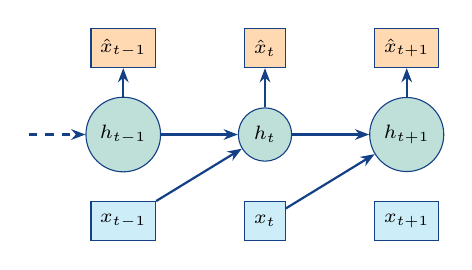
\begin{tikzpicture}[
					h/.style={circle, draw=UCMNavy, fill=AccentGreen!25, minimum size=0.6cm, font=\scriptsize},
					xb/.style={rectangle, draw=UCMNavy, fill=UCMBlue!20, minimum size=0.5cm, font=\scriptsize},
					a/.style={-{Stealth[length=1.8mm]}, UCMNavy, thick}
				]
				\foreach \t [count=\i from 0] in {t-1,t,t+1}{
					\node[h] (h\i) at (\i*1.8, 0) {$h_{\t}$};
					\node[xb] (x\i) at (\i*1.8, -1.1) {$x_{\t}$};
					\node[xb, fill=orange!30] (y\i) at (\i*1.8, 1.1) {$\hat{x}_{\t}$};
					\draw[a] (h\i) -- (y\i);
				}
				\draw[a] (h0) -- (h1); \draw[a] (h1) -- (h2);
				\draw[a] (x0) -- (h1); \draw[a] (x1) -- (h2);
				\draw[a, dashed] (-1.2,0) -- (h0);
			\end{tikzpicture}
		\end{column}
	\end{columns}

\end{frame}

\begin{frame}{Predicci\'on a $k$ Pasos: Los Errores se Acumulan}

	\begin{columns}[T]
		\begin{column}{0.52\textwidth}
			\small
			Experimento d2l: $x_t = \sin(0.01\,t) + 0.2\,\varepsilon_t$, $\varepsilon_t\sim\mathcal{N}(0,1)$, $T=1000$. Regresi\'on lineal con $\tau=4$ entradas, entrenada en los primeros 600 puntos.

			\vspace{0.1cm}

			\begin{itemize}
				\item \textbf{Un paso}: usar siempre valores observados. Excelente en toda la serie.
				\item \textbf{Varios pasos}: desde $t=604$ alimentar el modelo con sus propias predicciones:
			\end{itemize}
			\vspace{-0.1cm}
			\[\scriptstyle
				\begin{aligned}
					\hat{x}_{605} & = f(x_{601}, x_{602}, x_{603}, x_{604})                 \\
					\hat{x}_{606} & = f(x_{602}, x_{603}, x_{604}, \hat{x}_{605})           \\
					\hat{x}_{609} & = f(\hat{x}_{605}, \hat{x}_{606}, \hat{x}_{607}, \hat{x}_{608})
				\end{aligned}
			\]
			\vspace{-0.2cm}
			\begin{itemize}
				\item La predicci\'on decae a una constante en pocos pasos.
			\end{itemize}
		\end{column}

		\begin{column}{0.45\textwidth}
			\centering
			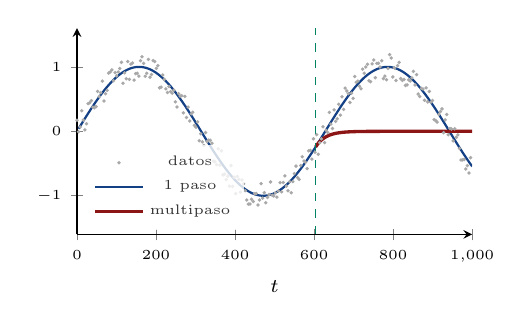
\begin{tikzpicture}
				\begin{axis}[
						width=6.6cm, height=4.2cm,
						xmin=0, xmax=1000, ymin=-1.6, ymax=1.6,
						xlabel={\scriptsize $t$}, tick label style={font=\tiny},
						legend style={font=\tiny, at={(0.02,0.02)}, anchor=south west, draw=none, fill=white, fill opacity=0.8},
						axis lines=left
					]
					\addplot[mitgray, only marks, mark size=0.4pt, samples=250, domain=0:1000] {sin(deg(0.01*x)) + 0.2*rand};
					\addlegendentry{datos}
					\addplot[UCMNavy, thick, samples=200, domain=4:1000] {sin(deg(0.01*x))};
					\addlegendentry{1 paso}
					\addplot[StanfordRed, very thick, samples=60, domain=604:1000] {sin(deg(6.04))*exp(-(x-604)/25)};
					\addlegendentry{multipaso}
					\draw[dashed, AccentGreen] (axis cs:604,-1.6) -- (axis cs:604,1.6);
				\end{axis}
			\end{tikzpicture}
			{\tiny Esquema cualitativo, adaptado de d2l \S9.1.}

			\begin{alertblock}{Lecciones}
				\scriptsize
				Interpolar es m\'as f\'acil que extrapolar. Nunca entrenar con datos del futuro. El error en $k$ pasos se compone: $\epsilon_2 = \bar\epsilon + c\,\epsilon_1$.
			\end{alertblock}
		\end{column}
	\end{columns}

\end{frame}

\begin{frame}{Texto como Secuencia: \textit{The Time Machine}}

	\begin{columns}[T]
		\begin{column}{0.5\textwidth}
			\small
			Corpus de d2l: \textit{The Time Machine} (H.\,G.\ Wells), poco m\'as de 30\,000 palabras.
			\begin{enumerate}
				\item Eliminar todo lo que no sea letra y pasar a min\'usculas:\\
				      {\scriptsize\texttt{re.sub('[\^{}A-Za-z]+', ' ', text).lower()}}
				\item Tokenizar a nivel de \textbf{car\'acter}.
				\item Vocabulario: \tok{<unk>}, espacio y 26 letras $\Rightarrow |\V| = 28$.
				\item Corpus: \textbf{173\,428} \'indices en una sola lista.
			\end{enumerate}

			\vspace{0.1cm}

			\begin{block}{Palabras vs.\ caracteres}
				\scriptsize
				Palabras: vocabulario grande, secuencias cortas. Caracteres: vocabulario m\'inimo, secuencias largas. Subpalabras (BPE): punto medio.
			\end{block}
		\end{column}

		\begin{column}{0.47\textwidth}
			\begin{block}{Frecuencias (a nivel de palabra)}
				\scriptsize
				\setlength{\tabcolsep}{3pt}
				\begin{tabular}{@{}lr@{\hspace{8pt}}lr@{}}
					\toprule
					\multicolumn{2}{c}{Unigramas} & \multicolumn{2}{c}{Trigramas} \\
					\midrule
					the & 2261 & the time traveller & 59 \\
					i & 1267 & the time machine & 30 \\
					and & 1245 & the medical man & 24 \\
					of & 1155 & it seemed to & 16 \\
					a & 816 & it was a & 15 \\
					\bottomrule
				\end{tabular}
			\end{block}

			\begin{block}{Ley de Zipf}
				\formula{\centering $n_i \propto \dfrac{1}{i^{\alpha}} \iff \log n_i = -\alpha \log i + c$}
				\scriptsize
				Tambi\'en vale para bigramas y trigramas. Consecuencia: la mayor\'ia de los $n$-gramas son \textbf{raros}, y contar no basta.
			\end{block}
		\end{column}
	\end{columns}

\end{frame}

\begin{frame}[shrink]{Modelos de Lenguaje}

	\begin{columns}[T]
		\begin{column}{0.5\textwidth}
			\small
			Un \textbf{modelo de lenguaje} estima $P(x_1,\ldots,x_T)$ y genera texto muestreando $x_t \sim P(x_t\mid x_{t-1},\ldots,x_1)$.

			\vspace{0.1cm}
			{\scriptsize $P(\text{deep, learning, is, fun}) = P(\text{deep})\,P(\text{learning}\mid\text{deep})\,P(\text{is}\mid\text{deep, learning})\,P(\text{fun}\mid\ldots)$}

			\begin{block}{Modelos de $n$-gramas}
				\scriptsize
				\begin{tabular}{@{}ll@{}}
					unigrama & $P(x_1)P(x_2)P(x_3)P(x_4)$ \\
					bigrama & $P(x_1)P(x_2\mid x_1)P(x_3\mid x_2)P(x_4\mid x_3)$ \\
					trigrama & $P(x_1)P(x_2\mid x_1)P(x_3\mid x_1,x_2)P(x_4\mid x_2,x_3)$
				\end{tabular}
				\\[3pt]
				Estimaci\'on por conteo: $\hat{P}(\text{learning}\mid\text{deep}) = \dfrac{n(\text{deep, learning})}{n(\text{deep})}$
			\end{block}
		\end{column}

		\begin{column}{0.47\textwidth}
			\begin{block}{Suavizado de Laplace}
				\scriptsize
				$n$: total de palabras; $m$: palabras distintas.
				\[
					\hat{P}(x) = \frac{n(x) + \epsilon_1/m}{n + \epsilon_1},\quad
					\hat{P}(x'\mid x) = \frac{n(x,x') + \epsilon_2\hat{P}(x')}{n(x) + \epsilon_2}
				\]
				Con $\epsilon_1 = 0$ no hay suavizado; con $\epsilon_1\to\infty$, $\hat{P}(x)\to 1/m$.
			\end{block}

			\begin{alertblock}{Limitaciones del conteo}
				\small
				\begin{itemize}
					\item Ley de Zipf: casi todos los $n$-gramas largos tienen conteo 0.
					\item Para un contexto de $n-1$ tokens, el n\'umero de par\'ametros crece como $|\V|^n$.
					\item No hay noci\'on de similitud: ``gato'' y ``felino'' son independientes.
				\end{itemize}
			\end{alertblock}
		\end{column}
	\end{columns}

\end{frame}

\begin{frame}{Perplejidad}

	\begin{columns}[T]
		\begin{column}{0.53\textwidth}
			\small
			Un buen modelo asigna \textbf{alta probabilidad} a los tokens que realmente ocurren. Entrop\'ia cruzada promedio sobre $n$ tokens:
			\[
				\frac{1}{n}\sum_{t=1}^{n} -\log P(x_t \mid x_{t-1},\ldots,x_1)
			\]
			\formula{\centering $\mathrm{PPL} = \exp\Big(-\dfrac{1}{n}\displaystyle\sum_{t=1}^{n}\log P(x_t \mid x_{t-1},\ldots,x_1)\Big)$}
			Interpretaci\'on: el n\'umero efectivo de opciones entre las que el modelo ``duda'' en cada paso.
		\end{column}

		\begin{column}{0.44\textwidth}
			\begin{block}{Valores de referencia}
				\small
				\begin{tabular}{@{}ll@{}}
					\toprule
					Modelo & PPL \\
					\midrule
					Perfecto (prob.\ 1) & 1 \\
					Uniforme sobre $\V$ & $|\V|$ \\
					Prob.\ 0 a un token real & $\infty$ \\
					\bottomrule
				\end{tabular}
				\\[3pt]
				\scriptsize Con caracteres, $|\V|=28$: un modelo \'util debe tener PPL muy por debajo de 28.
			\end{block}

			\begin{block}{Ejemplo cualitativo}
				\scriptsize
				Continuar ``It is raining\ldots'':\\
				\textit{outside} (buen modelo) $\cdot$ \textit{banana tree} (algo de estructura) $\cdot$ \textit{piouw;kcj pwepoiut} (modelo pobre)
			\end{block}
		\end{column}
	\end{columns}

\end{frame}

\begin{frame}{Particionar una Secuencia en Minilotes}

	\begin{columns}[c]
		\begin{column}{0.5\textwidth}
			\small
			El corpus es una sola secuencia de $T$ \'indices. Para entrenar un modelo de lenguaje:
			\begin{itemize}
				\item Cortar subsecuencias de largo $n$ (\texttt{num\_steps}).
				\item El \textbf{objetivo} es la misma ventana desplazada \textbf{un token}: $\mathbf{x}_t \to \mathbf{x}_{t+1}$.
				\item Un desplazamiento inicial aleatorio $d \in [0, n)$ en cada \'epoca var\'ia los cortes.
				\item Un minilote re\'une \texttt{batch\_size} subsecuencias.
			\end{itemize}

			\vspace{0.1cm}
			{\scriptsize En d2l: \texttt{X = array[:, :-1]}, \texttt{Y = array[:, 1:]} sobre ventanas de largo \texttt{num\_steps+1}.}
		\end{column}

		\begin{column}{0.47\textwidth}
			\centering
			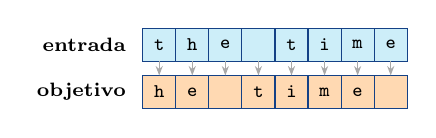
\begin{tikzpicture}[
					c/.style={draw=UCMNavy, minimum width=0.42cm, minimum height=0.42cm, font=\scriptsize\ttfamily, inner sep=0pt},
				]
				\node[font=\scriptsize\bfseries, anchor=east] at (-0.3, 0) {entrada};
				\node[font=\scriptsize\bfseries, anchor=east] at (-0.3, -0.6) {objetivo};
				\foreach \ch [count=\i from 0] in {t,h,e, ,t,i,m,e}{
					\node[c, fill=UCMBlue!20] at (\i*0.42, 0) {\ch};
				}
				\foreach \ch [count=\i from 0] in {h,e, ,t,i,m,e, }{
					\node[c, fill=orange!30] at (\i*0.42, -0.6) {\ch};
				}
				\foreach \i in {0,...,7}{\draw[-{Stealth[length=1.2mm]}, mitgray] (\i*0.42, -0.21) -- (\i*0.42, -0.39);}
			\end{tikzpicture}

			\vspace{0.4cm}

			\begin{block}{Ejemplo d2l, ejercicio de juguete}
				\scriptsize
				Fragmento ``machine'', lote 1: entrada \texttt{machin} $\to$ objetivo \texttt{achine}. En cada paso se predice el siguiente car\'acter con softmax + entrop\'ia cruzada.
			\end{block}
		\end{column}
	\end{columns}

\end{frame}

% =================================================================
\section{Redes Neuronales Recurrentes}

\begin{frame}[shrink]{De MLP a RNN: El Estado Oculto}

	\begin{columns}[T]
		\begin{column}{0.5\textwidth}
			\small
			Aproximar todo el historial con un \textbf{estado oculto}:
			\begin{gather*}
				P(x_t \mid x_{t-1},\ldots,x_1) \approx P(x_t \mid h_{t-1}),\\ h_t = f(x_t, h_{t-1})
			\end{gather*}

			\begin{block}{MLP (sin estado)}
				\small
				$\mathbf{H} = \phi(\mathbf{X}\W{xh} + \bvec{h})$, \quad $\mathbf{O} = \mathbf{H}\W{hq} + \bvec{q}$\\
				Cada entrada se procesa de forma independiente: sin memoria.
			\end{block}

			\begin{block}{RNN}
				\formula{\small $\mathbf{H}_t = \phi(\mathbf{X}_t\W{xh} + \mathbf{H}_{t-1}\W{hh} + \bvec{h})$\\[3pt]
					$\mathbf{O}_t = \mathbf{H}_t\W{hq} + \bvec{q}$}
			\end{block}
		\end{column}

		\begin{column}{0.47\textwidth}
			\begin{block}{Dimensiones (lote de $n$)}
				\scriptsize
				\begin{tabular}{@{}lll@{}}
					$\mathbf{X}_t \in \R^{n\times d}$ & $\W{xh} \in \R^{d\times h}$ & $\bvec{h} \in \R^{1\times h}$ \\
					$\mathbf{H}_t \in \R^{n\times h}$ & $\W{hh} \in \R^{h\times h}$ & \\
					$\mathbf{O}_t \in \R^{n\times q}$ & $\W{hq} \in \R^{h\times q}$ & $\bvec{q} \in \R^{1\times q}$
				\end{tabular}
			\end{block}

			\begin{itemize}
				\small
				\item Los \textbf{mismos par\'ametros} en todos los pasos: su n\'umero no crece con el largo de la secuencia.
				\item Equivale a concatenar entrada y estado:
				      \[\scriptstyle \mathbf{X}_t\W{xh} + \mathbf{H}_{t-1}\W{hh} = [\mathbf{X}_t, \mathbf{H}_{t-1}]\left[\begin{smallmatrix}\W{xh}\\ \W{hh}\end{smallmatrix}\right]\]
				\item $\phi$ suele ser $\tanh$.
			\end{itemize}
		\end{column}
	\end{columns}

\end{frame}

\begin{frame}{RNN Desenrollada en el Tiempo}

	\centering
	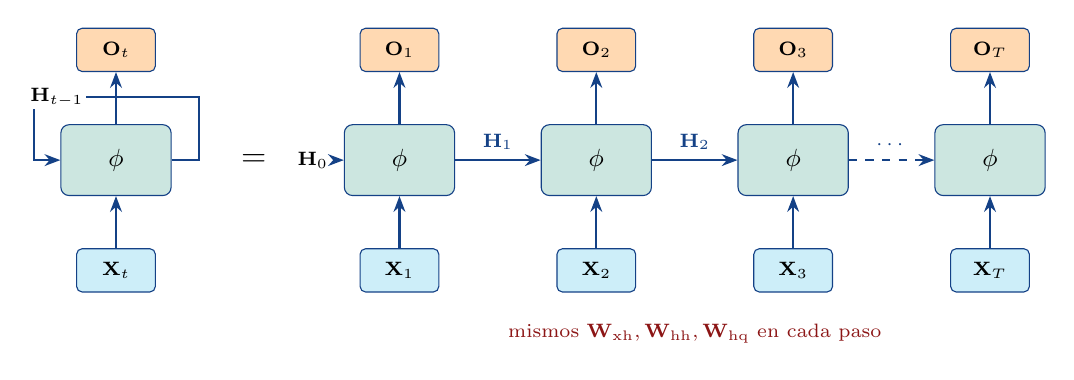
\begin{tikzpicture}[
			cell/.style={draw=UCMNavy, fill=AccentGreen!20, rounded corners=3pt, minimum width=1.4cm, minimum height=0.9cm, font=\small},
			xb/.style={draw=UCMNavy, fill=UCMBlue!20, rounded corners=2pt, minimum width=1cm, minimum height=0.55cm, font=\scriptsize},
			o/.style={draw=UCMNavy, fill=orange!30, rounded corners=2pt, minimum width=1cm, minimum height=0.55cm, font=\scriptsize},
			a/.style={-{Stealth[length=2mm]}, UCMNavy, thick}
		]
		% forma compacta
		\node[cell] (c) at (0,0) {$\phi$};
		\node[xb] (cx) at (0,-1.4) {$\mathbf{X}_t$};
		\node[o] (co) at (0,1.4) {$\mathbf{O}_t$};
		\draw[a] (cx) -- (c); \draw[a] (c) -- (co);
		\draw[a] (c.east) -- ++(0.35,0) -- ++(0,0.8) -- ++(-2.1,0) -- ++(0,-0.8) -- (c.west);
		\node[font=\scriptsize, fill=white, inner sep=1pt] at (-0.75,0.8) {$\mathbf{H}_{t-1}$};
		\node[font=\large] at (1.75,0) {$=$};

		% desenrollada
		\foreach \t/\l [count=\i from 0] in {1/1,2/2,3/3,4/T}{
			\node[cell] (u\i) at (3.6+\i*2.5, 0) {$\phi$};
			\node[xb] (x\i) at (3.6+\i*2.5, -1.4) {$\mathbf{X}_{\l}$};
			\node[o] (o\i) at (3.6+\i*2.5, 1.4) {$\mathbf{O}_{\l}$};
			\draw[a] (x\i) -- (u\i); \draw[a] (u\i) -- (o\i);
		}
		\node[font=\scriptsize] (h0) at (2.5,0) {$\mathbf{H}_0$};
		\draw[a] (h0) -- (u0);
		\draw[a] (u0) -- node[above, font=\scriptsize] {$\mathbf{H}_1$} (u1);
		\draw[a] (u1) -- node[above, font=\scriptsize] {$\mathbf{H}_2$} (u2);
		\draw[a, dashed] (u2) -- node[above, font=\scriptsize] {$\cdots$} (u3);
		\node[font=\scriptsize, text=StanfordRed] at (7.35,-2.2) {mismos $\W{xh}, \W{hh}, \W{hq}$ en cada paso};
	\end{tikzpicture}

	\vspace{0.3cm}

	\begin{columns}[T]
		\begin{column}{0.48\textwidth}
			\begin{block}{Modelo de lenguaje de caracteres}
				\small
				$\mathbf{X}_t$: one-hot del car\'acter $t$ ($d=|\V|=28$); $\mathbf{O}_t$: logits sobre el siguiente car\'acter ($q = |\V|$). P\'erdida: entrop\'ia cruzada en cada paso.
			\end{block}
		\end{column}
		\begin{column}{0.48\textwidth}
			\begin{block}{Clasificaci\'on de una secuencia}
				\small
				Se ignoran las salidas intermedias y se clasifica con $\mathbf{H}_T$ (o el promedio de los $\mathbf{H}_t$). Es el caso de AG\_NEWS.
			\end{block}
		\end{column}
	\end{columns}

\end{frame}

\begin{frame}[fragile]{RNN desde Cero}

	\begin{columns}[T]
		\begin{column}{0.58\textwidth}
			\begin{tcolorbox}[codebox]
\scriptsize
\begin{verbatim}
class RNNScratch(nn.Module):
    def __init__(self, num_inputs, num_hiddens,
                 sigma=0.01):
        super().__init__()
        self.W_xh = nn.Parameter(
            torch.randn(num_inputs, num_hiddens)*sigma)
        self.W_hh = nn.Parameter(
            torch.randn(num_hiddens, num_hiddens)*sigma)
        self.b_h = nn.Parameter(
            torch.zeros(num_hiddens))

    def forward(self, inputs, state=None):
        # inputs: (num_steps, batch, num_inputs)
        if state is None:
            state = torch.zeros((inputs.shape[1],
                                 self.W_hh.shape[0]))
        outputs = []
        for X in inputs:           # bucle en el tiempo
            state = torch.tanh(X @ self.W_xh +
                        state @ self.W_hh + self.b_h)
            outputs.append(state)
        return outputs, state
\end{verbatim}
			\end{tcolorbox}
		\end{column}

		\begin{column}{0.39\textwidth}
			\begin{block}{Configuraci\'on d2l (Time Machine)}
				\small
				\begin{tabular}{@{}ll@{}}
					\texttt{batch\_size} & 1024 \\
					\texttt{num\_steps} & 32 \\
					\texttt{num\_hiddens} & 32 \\
					tasa de aprendizaje & 1 \\
					\'epocas & 100 \\
					recorte de gradiente $\theta$ & 1 \\
				\end{tabular}
			\end{block}

			\begin{block}{Generar texto}
				\small
				Calentar el estado con un prefijo y luego tomar el car\'acter m\'as probable, realimentarlo y repetir:\\[2pt]
				\scriptsize
				Antes de entrenar: \texttt{it hasoadd dd dd dd dd dd}\\
				Despu\'es: \texttt{it has and the trave the t}
			\end{block}
		\end{column}
	\end{columns}

\end{frame}

\begin{frame}{Retropropagaci\'on a Trav\'es del Tiempo (BPTT)}

	\begin{columns}[T]
		\begin{column}{0.53\textwidth}
			\small
			Modelo simplificado: $h_t = f(x_t, h_{t-1}, w_h)$, $o_t = g(h_t, w_o)$, $L = \frac{1}{T}\sum_t l(y_t, o_t)$.
			\[
				\frac{\partial L}{\partial w_h} = \frac{1}{T}\sum_{t=1}^{T}\frac{\partial l(y_t,o_t)}{\partial o_t}\,\frac{\partial g(h_t,w_o)}{\partial h_t}\,\frac{\partial h_t}{\partial w_h}
			\]
			El t\'ermino dif\'icil es recursivo, porque $h_{t-1}$ tambi\'en depende de $w_h$:
			\[
				\frac{\partial h_t}{\partial w_h} = \frac{\partial f(x_t,h_{t-1},w_h)}{\partial w_h} + \frac{\partial f(x_t,h_{t-1},w_h)}{\partial h_{t-1}}\,\frac{\partial h_{t-1}}{\partial w_h}
			\]
			Desenrollando:
			\formula{\small $\dfrac{\partial h_t}{\partial w_h} = \dfrac{\partial f_t}{\partial w_h} + \displaystyle\sum_{i=1}^{t-1}\Bigg(\prod_{j=i+1}^{t}\dfrac{\partial f_j}{\partial h_{j-1}}\Bigg)\dfrac{\partial f_i}{\partial w_h}$}
		\end{column}

		\begin{column}{0.44\textwidth}
			\begin{alertblock}{El producto largo}
				\small
				El aporte del paso $i$ al gradiente en $t$ pasa por un \textbf{producto de $t-i$ jacobianos}. Con secuencias de cientos o miles de pasos:
				\begin{itemize}
					\item factores $<1$ $\Rightarrow$ \textbf{se desvanece};
					\item factores $>1$ $\Rightarrow$ \textbf{explota}.
				\end{itemize}
			\end{alertblock}

			\begin{block}{Caso lineal}
				\small
				Con $\mathbf{h}_t = \W{hx}\mathbf{x}_t + \W{hh}\mathbf{h}_{t-1}$:
				\[
					\frac{\partial L}{\partial \mathbf{h}_t} = \sum_{i=t}^{T}\left(\W{hh}^\top\right)^{T-i}\W{qh}^\top\frac{\partial L}{\partial \mathbf{o}_{T+t-i}}
				\]
				Potencias de $\W{hh}^\top$: valores propios $|\lambda|<1$ se anulan, $|\lambda|>1$ divergen.
			\end{block}
		\end{column}
	\end{columns}

\end{frame}

\begin{frame}[shrink]{Truncamiento y Recorte de Gradientes}

	\begin{columns}[T]
		\begin{column}{0.5\textwidth}
			\begin{block}{Estrategias de BPTT}
				\small
				\begin{enumerate}
					\item \textbf{Completo}: sumar todos los t\'erminos. Lento e inestable; casi nunca se usa.
					\item \textbf{Truncado}: cortar la suma tras $\tau$ pasos (en la pr\'actica, \texttt{num\_steps} y \texttt{detach()} del estado). Aproximado pero estable; act\'ua como regularizador hacia dependencias cortas.
					\item \textbf{Aleatorio}: reemplazar el t\'ermino recursivo por $\xi_t$ con $P(\xi_t=0)=1-\pi_t$, $P(\xi_t=\pi_t^{-1})=\pi_t$, as\'i $\mathbb{E}[\xi_t]=1$. En la pr\'actica no supera al truncado.
				\end{enumerate}
			\end{block}

			\centering
			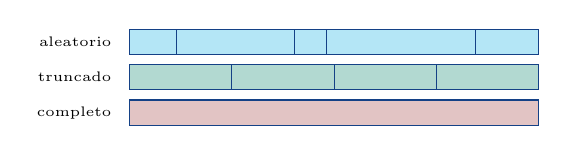
\begin{tikzpicture}[s/.style={draw=UCMNavy, minimum height=0.32cm, inner sep=0pt}]
				\node[font=\tiny, anchor=east] at (-0.1,0.9) {aleatorio};
				\node[font=\tiny, anchor=east] at (-0.1,0.45) {truncado};
				\node[font=\tiny, anchor=east] at (-0.1,0) {completo};
				\foreach \a/\b in {0/0.6,0.6/2.1,2.1/2.5,2.5/4.4,4.4/5.2}{\node[s, fill=UCMBlue!30, minimum width=(\b-\a)*1cm, anchor=west] at (\a,0.9) {};}
				\foreach \a in {0,1.3,2.6,3.9}{\node[s, fill=AccentGreen!30, minimum width=1.3cm, anchor=west] at (\a,0.45) {};}
				\node[s, fill=StanfordRed!25, minimum width=5.2cm, anchor=west] at (0,0) {};
			\end{tikzpicture}
		\end{column}

		\begin{column}{0.47\textwidth}
			\begin{block}{Recorte de gradientes}
				\small
				Contra la \textbf{explosi\'on}: proyectar el gradiente (de todos los par\'ametros concatenados) a una bola de radio $\theta$:
				\formula{\centering $\mathbf{g} \leftarrow \min\Big(1, \dfrac{\theta}{\|\mathbf{g}\|}\Big)\,\mathbf{g}$}
				Conserva la direcci\'on, acota la magnitud. En PyTorch:\\
				{\scriptsize\texttt{torch.nn.utils.clip\_grad\_norm\_(net.parameters(), 1)}}
			\end{block}

			\begin{alertblock}{Pero\ldots}
				\small
				El recorte \textbf{no} resuelve el \textbf{desvanecimiento}: la RNN simple olvida lo que vio hace muchos pasos. Soluci\'on: \textbf{compuertas} (LSTM, GRU).
			\end{alertblock}
		\end{column}
	\end{columns}

\end{frame}

% =================================================================
\section{RNN con Compuertas}

\begin{frame}{Long Short-Term Memory (LSTM)}

	\begin{columns}[c]
		\begin{column}{0.5\textwidth}
			\centering
			\resizebox{\linewidth}{!}{%
	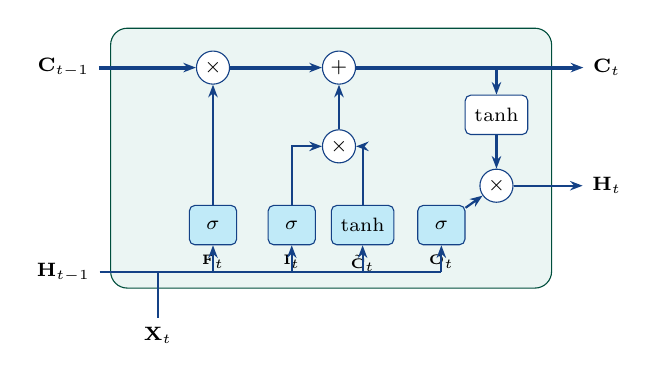
\begin{tikzpicture}[
					g/.style={draw=UCMNavy, fill=UCMBlue!25, rounded corners=2pt, minimum width=0.6cm, minimum height=0.5cm, font=\scriptsize},
					op/.style={circle, draw=UCMNavy, fill=white, minimum size=0.42cm, inner sep=0pt, font=\scriptsize},
					a/.style={-{Stealth[length=1.6mm]}, UCMNavy, thick}
				]
				\draw[rounded corners=6pt, fill=AccentGreen!8, draw=AccentGreen!60!black] (-0.3,-0.3) rectangle (5.3,3.0);
				% linea de memoria
				\node[font=\scriptsize] (cin) at (-0.9,2.5) {$\mathbf{C}_{t-1}$};
				\node[op] (m1) at (1.0,2.5) {$\times$};
				\node[op] (p1) at (2.6,2.5) {$+$};
				\node[font=\scriptsize] (cout) at (6.0,2.5) {$\mathbf{C}_t$};
				\draw[a, line width=1.4pt] (cin) -- (m1); \draw[a, line width=1.4pt] (m1) -- (p1); \draw[a, line width=1.4pt] (p1) -- (cout);
				% compuertas
				\node[g] (f) at (1.0,0.5) {$\sigma$};
				\node[g] (i) at (2.0,0.5) {$\sigma$};
				\node[g] (cc) at (2.9,0.5) {$\tanh$};
				\node[g] (o) at (3.9,0.5) {$\sigma$};
				\node[font=\tiny, below=0pt of f] {$\mathbf{F}_t$};
				\node[font=\tiny, below=0pt of i] {$\mathbf{I}_t$};
				\node[font=\tiny, below=0pt of cc] {$\tilde{\mathbf{C}}_t$};
				\node[font=\tiny, below=0pt of o] {$\mathbf{O}_t$};
				\node[op] (m2) at (2.6,1.5) {$\times$};
				\draw[a] (f) -- (m1);
				\draw[a] (i) |- (m2); \draw[a] (cc) |- (m2);
				\draw[a] (m2) -- (p1);
				% salida
				\node[g, fill=white] (th) at (4.6,1.9) {$\tanh$};
				\node[op] (m3) at (4.6,1.0) {$\times$};
				\draw[a] (4.6,2.5) -- (th); \draw[a] (th) -- (m3); \draw[a] (o) -- (m3);
				\node[font=\scriptsize] (hout) at (6.0,1.0) {$\mathbf{H}_t$};
				\draw[a] (m3) -- (hout);
				% entradas
				\node[font=\scriptsize] (hin) at (-0.9,-0.1) {$\mathbf{H}_{t-1}$};
				\node[font=\scriptsize] (xin) at (0.3,-0.9) {$\mathbf{X}_t$};
				\draw[UCMNavy, thick] (hin) -- (0.3,-0.1);
				\draw[UCMNavy, thick] (xin) -- (0.3,-0.1) -- (3.9,-0.1);
				\foreach \n in {f,i,cc,o}{\draw[a] (\n |- 0,-0.1) -- (\n.south);}
			\end{tikzpicture}}
		\end{column}

		\begin{column}{0.47\textwidth}
			\small
			Dos estados: la \textbf{celda de memoria} $\mathbf{C}_t$ y el estado oculto $\mathbf{H}_t$. Tres compuertas con sigmoide (valores en $[0,1]$, act\'uan como m\'ascaras):
			\formula{\scriptsize
				$\begin{aligned}
						\mathbf{F}_t       & = \sigma(\mathbf{X}_t\W{xf} + \mathbf{H}_{t-1}\W{hf} + \bvec{f}) & \text{olvido} \\
						\mathbf{I}_t       & = \sigma(\mathbf{X}_t\W{xi} + \mathbf{H}_{t-1}\W{hi} + \bvec{i}) & \text{entrada} \\
						\mathbf{O}_t       & = \sigma(\mathbf{X}_t\W{xo} + \mathbf{H}_{t-1}\W{ho} + \bvec{o}) & \text{salida} \\
						\tilde{\mathbf{C}}_t & = \tanh(\mathbf{X}_t\W{xc} + \mathbf{H}_{t-1}\W{hc} + \bvec{c}) &               \\
						\mathbf{C}_t       & = \mathbf{F}_t\odot\mathbf{C}_{t-1} + \mathbf{I}_t\odot\tilde{\mathbf{C}}_t &  \\
						\mathbf{H}_t       & = \mathbf{O}_t\odot\tanh(\mathbf{C}_t) &
					\end{aligned}$}
			La actualizaci\'on de $\mathbf{C}_t$ es \textbf{aditiva}: si $\mathbf{F}_t\approx 1$, el gradiente fluye sin atenuarse.
		\end{column}
	\end{columns}

\end{frame}

\begin{frame}{Intuici\'on de las Compuertas y la GRU}

	\begin{columns}[T]
		\begin{column}{0.5\textwidth}
			\begin{block}{La memoria como banderas}
				\small
				Las componentes de $\mathbf{C}_t$ pueden verse como \emph{banderas} que se encienden y apagan:
				\begin{itemize}
					\item Al leer ``\textit{Alice}'': encender ``sujeto femenino''.
					\item Al leer ``\textit{and Tom}'': encender ``sujeto plural''.
					\item Al leer ``\textit{not}'': invertir la polaridad de lo que sigue.
				\end{itemize}
				La compuerta de \textbf{olvido} decide qu\'e banderas mantener; la de \textbf{entrada}, qu\'e escribir; la de \textbf{salida}, qu\'e mostrar en $\mathbf{H}_t$.
			\end{block}
		\end{column}

		\begin{column}{0.47\textwidth}
			\begin{block}{Gated Recurrent Unit (GRU)}
				\small
				Versi\'on simplificada: un solo estado y dos compuertas.
				\formula{\scriptsize
					$\begin{aligned}
							\mathbf{R}_t & = \sigma(\mathbf{X}_t\W{xr} + \mathbf{H}_{t-1}\W{hr} + \bvec{r}) \\
							\mathbf{Z}_t & = \sigma(\mathbf{X}_t\W{xz} + \mathbf{H}_{t-1}\W{hz} + \bvec{z}) \\
							\tilde{\mathbf{H}}_t & = \tanh(\mathbf{X}_t\W{xh} + (\mathbf{R}_t\odot\mathbf{H}_{t-1})\W{hh} + \bvec{h}) \\
							\mathbf{H}_t & = \mathbf{Z}_t\odot\mathbf{H}_{t-1} + (1-\mathbf{Z}_t)\odot\tilde{\mathbf{H}}_t
						\end{aligned}$}
				$\mathbf{R}_t$ (reinicio) decide cu\'anto pasado usar; $\mathbf{Z}_t$ (actualizaci\'on), cu\'anto copiar. Menos par\'ametros que LSTM, desempe\~no similar.
			\end{block}
		\end{column}
	\end{columns}

\end{frame}

\begin{frame}{RNN Bidireccionales y Multicapa}

	\begin{columns}[T]
		\begin{column}{0.5\textwidth}
			\centering
			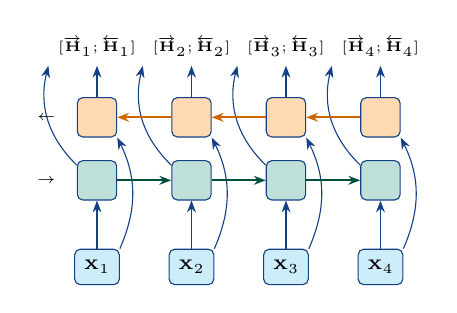
\begin{tikzpicture}[
					f/.style={draw=UCMNavy, fill=AccentGreen!25, rounded corners=2pt, minimum size=0.5cm},
					b/.style={draw=UCMNavy, fill=orange!30, rounded corners=2pt, minimum size=0.5cm},
					xb/.style={draw=UCMNavy, fill=UCMBlue!20, rounded corners=2pt, minimum size=0.45cm, font=\tiny},
					a/.style={-{Stealth[length=1.5mm]}, UCMNavy}
				]
				\foreach \i in {1,2,3,4}{
					\node[xb] (x\i) at (\i*1.2,-1.1) {$\mathbf{X}_{\i}$};
					\node[f] (f\i) at (\i*1.2,0) {};
					\node[b] (b\i) at (\i*1.2,0.8) {};
					\node[font=\tiny] (y\i) at (\i*1.2,1.7) {$[\overrightarrow{\mathbf{H}}_{\i};\overleftarrow{\mathbf{H}}_{\i}]$};
					\draw[a] (x\i) -- (f\i);
					\draw[a] (x\i.north east) to[bend right=25] (b\i.south east);
					\draw[a] (f\i) to[bend left=30] (y\i.south west);
					\draw[a] (b\i) -- (y\i);
				}
				\foreach \i/\j in {1/2,2/3,3/4}{\draw[a, thick, AccentGreen!60!black] (f\i) -- (f\j); \draw[a, thick, orange!80!black] (b\j) -- (b\i);}
				\node[font=\tiny, anchor=east] at (0.8,0) {$\rightarrow$};
				\node[font=\tiny, anchor=east] at (0.8,0.8) {$\leftarrow$};
			\end{tikzpicture}

			\small
			\begin{itemize}
				\item Dos RNN: una lee de izquierda a derecha, otra al rev\'es. Se concatenan sus estados.
				\item \'Util cuando toda la secuencia est\'a disponible (clasificaci\'on, etiquetado). \textbf{No} sirve para generar texto.
				\item \texttt{bidirectional=True}: la salida tiene tama\~no $2h$.
			\end{itemize}
		\end{column}

		\begin{column}{0.47\textwidth}
			\begin{block}{RNN multicapa (apiladas)}
				\small
				La secuencia de salidas de una capa es la entrada de la siguiente:
				\[
					\mathbf{H}_t^{(\ell)} = \phi\big(\mathbf{H}_t^{(\ell-1)}\W{xh}^{(\ell)} + \mathbf{H}_{t-1}^{(\ell)}\W{hh}^{(\ell)} + \bvec{h}^{(\ell)}\big)
				\]
				con $\mathbf{H}_t^{(0)} = \mathbf{X}_t$. Como en las CNN, las capas altas capturan patrones de mayor nivel.\\[3pt]
				\texttt{num\_layers=L}: el estado final \texttt{h} tiene forma $(L\cdot\text{dirs}, B, h)$.
			\end{block}

			\begin{block}{En PyTorch}
				\scriptsize
				\texttt{nn.LSTM(embed\_dim, hidden\_dim, num\_layers=2,}\\
				\texttt{\ \ \ \ \ \ \ \ bidirectional=True, batch\_first=True)}
			\end{block}
		\end{column}
	\end{columns}

\end{frame}

% =================================================================
\section{Laboratorio: Clasificaci\'on con RNN}

\begin{frame}[fragile]{Clasificador RNN y LSTM (Lab 3.2)}

	\begin{columns}[T]
		\begin{column}{0.5\textwidth}
			\begin{tcolorbox}[codebox]
\scriptsize
\begin{verbatim}
class RNNClassifier(nn.Module):
  def __init__(self, vocab_size, embed_dim,
               hidden_dim, num_class):
    super().__init__()
    self.embedding = nn.Embedding(vocab_size,
                                  embed_dim)
    self.rnn = nn.RNN(embed_dim, hidden_dim,
                      batch_first=True)
    self.fc = nn.Linear(hidden_dim, num_class)

  def forward(self, x):         # (B, T)
    x = self.embedding(x)       # (B, T, d)
    x, h = self.rnn(x)          # x: (B, T, h)
    return self.fc(x.mean(dim=1))
\end{verbatim}
			\end{tcolorbox}
		\end{column}

		\begin{column}{0.47\textwidth}
			\begin{tcolorbox}[codebox]
\scriptsize
\begin{verbatim}
class LSTMClassifier(nn.Module):
  # ... igual, pero:
  self.rnn = nn.LSTM(embed_dim, hidden_dim,
                     batch_first=True)
  def forward(self, x):
    x = self.embedding(x)
    x, (h, c) = self.rnn(x)
    return self.fc(h[-1])   # ultimo estado
\end{verbatim}
			\end{tcolorbox}

			\begin{block}{Salidas de \texttt{nn.RNN} / \texttt{nn.LSTM}}
				\small
				\begin{itemize}
					\item \texttt{x}: estados en \textbf{todos} los pasos, $(B, T, h)$.
					\item \texttt{h}: estado \textbf{final} por capa, $(L, B, h)$.
					\item LSTM devuelve adem\'as la celda \texttt{c}.
				\end{itemize}
			\end{block}

			{\small Configuraci\'on: $d=64$, $h=32$, lote 16, Adam $\eta=10^{-3}$, una \'epoca.}
		\end{column}
	\end{columns}

\end{frame}

\begin{frame}[fragile]{Secuencias Empaquetadas}

	\begin{columns}[T]
		\begin{column}{0.5\textwidth}
			\small
			Con relleno, la RNN ejecuta pasos sobre ceros que no aportan informaci\'on, y en \texttt{h[-1]} el \'ultimo estado corresponde al relleno, no al \'ultimo token real.

			\vspace{0.2cm}
			\centering
			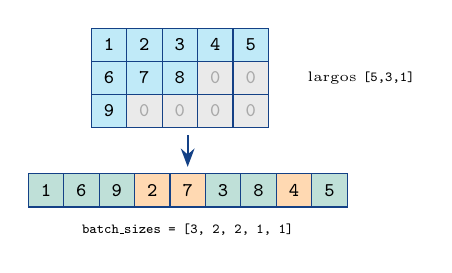
\begin{tikzpicture}[
					c/.style={draw=UCMNavy, minimum width=0.45cm, minimum height=0.42cm, font=\scriptsize\ttfamily, inner sep=0pt},
					p/.style={c, fill=mitgray!25, text=mitgray}
				]
				\foreach \r/\vals/\n in {0/{1,2,3,4,5}/5, 1/{6,7,8,0,0}/3, 2/{9,0,0,0,0}/1}{
					\foreach \v [count=\c from 0] in \vals{
						\ifnum\c<\n \node[c, fill=UCMBlue!25] at (\c*0.45, -\r*0.42) {\v};
						\else \node[p] at (\c*0.45, -\r*0.42) {\v}; \fi
					}
				}
				\node[font=\tiny, anchor=west] at (2.4,-0.42) {largos \texttt{[5,3,1]}};
				\draw[-{Stealth}, thick, UCMNavy] (1,-1.15) -- (1,-1.55);
				\foreach \v/\g [count=\c from 0] in {1/0,6/0,9/0,2/1,7/1,3/2,8/2,4/3,5/4}{
					\pgfmathsetmacro{\col}{mod(\g,2)==0 ? "AccentGreen!25" : "orange!30"}
					\node[c, fill=\col] at (-0.8+\c*0.45, -1.85) {\v};
				}
				\node[font=\tiny] at (1,-2.35) {\texttt{batch\_sizes = [3, 2, 2, 1, 1]}};
			\end{tikzpicture}

			\raggedright
			\scriptsize
			El paso 1 procesa un minilote de 3, los pasos 2--3 de 2, y los pasos 4--5 de 1.
		\end{column}

		\begin{column}{0.47\textwidth}
			\begin{tcolorbox}[codebox]
\scriptsize
\begin{verbatim}
def forward(self, x, lengths):
    x = self.embedding(x)
    px = nn.utils.rnn.pack_padded_sequence(
             x, lengths, batch_first=True,
             enforce_sorted=False)
    px, (h, c) = self.rnn(px)
    # opcional, si se usan las salidas:
    x, _ = nn.utils.rnn.pad_packed_sequence(
               px, batch_first=True)
    return self.fc(h[-1])
\end{verbatim}
			\end{tcolorbox}

			\begin{itemize}
				\small
				\item El \emph{collate} (\texttt{pad\_length}) devuelve tambi\'en los largos.
				\item \texttt{lengths} debe estar en \textbf{CPU}.
				\item \texttt{h[-1]} es ahora el estado tras el \'ultimo token \emph{real} de cada secuencia.
			\end{itemize}
		\end{column}
	\end{columns}

\end{frame}

\begin{frame}{Resultados en AG\_NEWS (una \'epoca)}

	\begin{columns}[c]
		\begin{column}{0.55\textwidth}
			\centering
			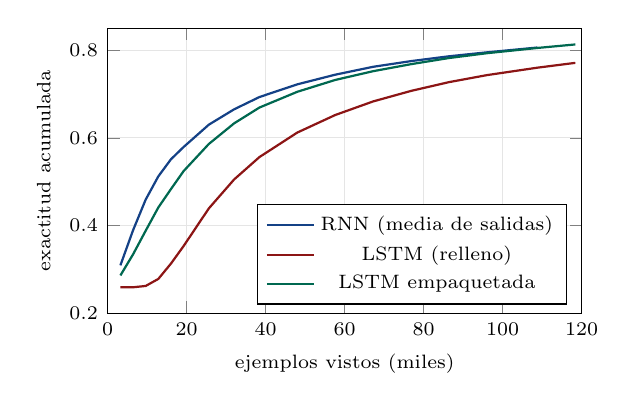
\begin{tikzpicture}
				\begin{axis}[
						width=7.6cm, height=5.2cm,
						xlabel={\scriptsize ejemplos vistos (miles)}, ylabel={\scriptsize exactitud acumulada},
						xmin=0, xmax=120, ymin=0.2, ymax=0.85,
						tick label style={font=\scriptsize},
						legend style={font=\scriptsize, at={(0.97,0.03)}, anchor=south east},
						grid=major, grid style={mitgray!30}
					]
					\addplot[UCMNavy, thick, mark=none] coordinates {(3.2,0.309) (6.4,0.389) (9.6,0.459) (12.8,0.512) (16,0.551) (19.2,0.579) (25.6,0.630) (32,0.665) (38.4,0.693) (48,0.722) (57.6,0.744) (67.2,0.762) (76.8,0.775) (86.4,0.786) (96,0.795) (108.8,0.806)};
					\addlegendentry{RNN (media de salidas)}
					\addplot[StanfordRed, thick, mark=none] coordinates {(3.2,0.259) (6.4,0.259) (9.6,0.262) (12.8,0.278) (16,0.313) (19.2,0.353) (25.6,0.439) (32,0.505) (38.4,0.556) (48,0.612) (57.6,0.652) (67.2,0.683) (76.8,0.707) (86.4,0.727) (96,0.743) (108.8,0.760) (118.4,0.771)};
					\addlegendentry{LSTM (relleno)}
					\addplot[AccentGreen!80!black, thick, mark=none] coordinates {(3.2,0.286) (6.4,0.334) (9.6,0.388) (12.8,0.441) (16,0.483) (19.2,0.524) (25.6,0.586) (32,0.633) (38.4,0.669) (48,0.705) (57.6,0.732) (67.2,0.752) (76.8,0.768) (86.4,0.782) (96,0.793) (108.8,0.805) (118.4,0.813)};
					\addlegendentry{LSTM empaquetada}
				\end{axis}
			\end{tikzpicture}
		\end{column}

		\begin{column}{0.42\textwidth}
			\small
			\begin{itemize}
				\item La LSTM con relleno tarda en arrancar ($\approx 26\%$, azar con 4 clases, durante los primeros 10\,000 ejemplos): \texttt{h[-1]} ve sobre todo ceros de relleno.
				\item Empaquetar corrige eso: misma red, \textbf{81.4\%} frente a 77.3\%.
				\item La RNN simple con promedio de salidas llega a $\approx 80.6\%$.
				\item Todas quedan por debajo del BoW lineal (86\%) tras una \'epoca: las RNN son \textbf{lentas de entrenar}; necesitan m\'as \'epocas, GPU y tasa de aprendizaje peque\~na.
			\end{itemize}

			\vspace{0.1cm}
			{\scriptsize Exactitud de entrenamiento acumulada, tomada de las salidas del notebook.}
		\end{column}
	\end{columns}

\end{frame}

% =================================================================
\section{Conclusiones}

\begin{frame}{Conclusiones}

	\begin{itemize}
		\item Una capa de \textbf{embedding} es una tabla de b\'usqueda entrenable ($\equiv$ one-hot $\times$ matriz). Puede inicializarse con word2vec/GloVe y congelarse o ajustarse.

		\vspace{0.12cm}

		\item Promediar embeddings (\texttt{EmbeddingBag}) es r\'apido pero \textbf{ignora el orden}.

		\vspace{0.12cm}

		\item Un \textbf{modelo de lenguaje} factoriza $P(x_1,\ldots,x_T)$ autorregresivamente; los $n$-gramas sufren de dispersi\'on (Zipf). Se eval\'ua con \textbf{perplejidad}.

		\vspace{0.12cm}

		\item Una \textbf{RNN} resume el pasado en un estado oculto $\mathbf{H}_t$ con par\'ametros compartidos en el tiempo, y se entrena con \textbf{BPTT}.

		\vspace{0.12cm}

		\item Los productos de jacobianos causan gradientes que \textbf{explotan} (recorte) o \textbf{se desvanecen} (compuertas: \textbf{LSTM}, \textbf{GRU}).

		\vspace{0.12cm}

		\item En la pr\'actica: empaquetar secuencias, usar variantes bidireccionales y multicapa.
	\end{itemize}

	\vspace{0.15cm}

	\begin{alertblock}{Para el laboratorio 3.2}
		Entrenar RNN, LSTM y LSTM empaquetada en AG\_NEWS. Probar \texttt{bidirectional=True}, \texttt{num\_layers=2} y una GRU; inicializar el embedding con vectores preentrenados y comparar contra el BoW de la clase 3.1.
	\end{alertblock}

\end{frame}

\begin{frame}{Referencias}

	\small
	\begin{itemize}
		\item A.\ Zhang, Z.\ C.\ Lipton, M.\ Li \& A.\ J.\ Smola, \textit{Dive into Deep Learning}, Cambridge University Press, 2023. Cap.\ 9: \textit{Recurrent Neural Networks}; Cap.\ 10: \textit{Modern Recurrent Neural Networks}. \texttt{d2l.ai}
		\item S.\ Hochreiter \& J.\ Schmidhuber, ``Long Short-Term Memory'', \textit{Neural Computation} 9(8), 1997.
		\item K.\ Cho et al., ``Learning Phrase Representations using RNN Encoder--Decoder for Statistical Machine Translation'' (GRU), EMNLP 2014.
		\item Y.\ Bengio, P.\ Simard \& P.\ Frasconi, ``Learning Long-Term Dependencies with Gradient Descent is Difficult'', \textit{IEEE Trans.\ Neural Networks}, 1994.
		\item R.\ Pascanu, T.\ Mikolov \& Y.\ Bengio, ``On the Difficulty of Training Recurrent Neural Networks'', ICML 2013.
		\item M.\ Schuster \& K.\ K.\ Paliwal, ``Bidirectional Recurrent Neural Networks'', \textit{IEEE Trans.\ Signal Processing}, 1997.
		\item C.\ Olah, ``Understanding LSTM Networks'', 2015. \texttt{colah.github.io/posts/2015-08-Understanding-LSTMs}
		\item T.\ Mikolov et al., ``Distributed Representations of Words and Phrases and their Compositionality'', NeurIPS 2013.
	\end{itemize}

\end{frame}

\end{document}
